\documentclass[10pt]{article}
\usepackage[polish]{babel}
\usepackage[utf8]{inputenc}
\usepackage[T1]{fontenc}
\usepackage{amsmath}
\usepackage{amsfonts}
\usepackage{amssymb}
\usepackage[version=4]{mhchem}
\usepackage{stmaryrd}
\usepackage{graphicx}
\usepackage[export]{adjustbox}
\graphicspath{ {./images/} }

\begin{document}
\(\qquad\)

\section*{Instrukcja dla zdającego}
\begin{enumerate}
  \item Sprawdź, czy arkusz zawiera 16 stron. Ewentualny brak zgłoś przewodniczącemu zespołu nadzorującego egzamin.
  \item Rozwiązania zadań i odpowiedzi zamieść w miejscu na to przeznaczonym.
  \item Odpowiedzi do zadań zamkniętych (1-25) przenieś na kartę odpowiedzi, zaznaczając je w części karty przeznaczonej dla zdającego. Zamaluj pola do tego przeznaczone. Błędne zaznaczenie otocz kółkiem i zaznacz właściwe.
  \item Pamiętaj, że pominięcie argumentacji lub istotnych obliczeń w rozwiązaniu zadania otwartego (26-34) może spowodować, że za to rozwiązanie nie otrzymasz pełnej liczby punktów.
  \item Pisz czytelnie i używaj tylko długopisu lub pióra z czarnym tuszem lub atramentem.
  \item Nie używaj korektora, a błędne zapisy wyraźnie przekreśl.
  \item Pamiętaj, że zapisy w brudnopisie nie będą oceniane.
  \item Możesz korzystać z zestawu wzorów matematycznych, cyrkla i linijki oraz kalkulatora prostego.
  \item Na tej stronie oraz na karcie odpowiedzi wpisz swój kod (nazwisko i imie - zgodnie z ustaleniami szkolnymi).
  \item Nie wpisuj żadnych znaków w części przeznaczonej dla egzaminatora.
\end{enumerate}

Życzymy powodzenia!

Liczba punktów\\
do uzyskania: \(\mathbf{5 0}\)

Zadanie 1. (1p)\\
Wartość wyrażenia \(\left(\frac{2^{-2} \cdot \sqrt[4]{16}}{4^{\frac{1}{2}} \cdot\left(\frac{1}{2}\right)^{-3}}\right)^{-1}\) jest równa\\
A. \(2^{5}\)\\
B. \(2^{-5}\)\\
C. \(2^{-4}\)\\
D. \(2^{4}\)

Zadanie 2. (1p)\\
Różnica liczby \(x\) i jej kwadratu jest najmniejsza dla liczby \(x\) równej\\
A. -1\\
B. 1\\
C. \(-\frac{1}{2}\)\\
D. \(\frac{1}{2}\)

Zadanie 3. (1p)\\
Iloczyn liczby \(\sqrt{2}\) i odwrotności liczby \(\sqrt{2}+1\) jest równy\\
A. \(2+\sqrt{2}\)\\
B. \(2-\sqrt{2}\)\\
C. \(2+2 \sqrt{2}\)\\
D. \(2-2 \sqrt{2}\)

\section*{Zadanie 4. (1p)}
Cenę roweru obniżono o \(20 \%\), a po miesiącu podniesiono o \(10 \%\). W wyniku obu operacji finansowych cena roweru zmniejszyła się o\\
A. \(10 \%\)\\
B. \(11 \%\)\\
C. \(12 \%\)\\
D. \(15 \%\)

Zadanie 5. (1p)\\
Wartość liczbowa wyrażenia \(\log _{2} 16+\log _{2} 8-4 \log _{2} 2\) jest równa\\
A. 1\\
B. 2\\
C. 3\\
D. 4

Zadanie 6. (1p)\\
Jeśli miejscem zerowym funkcji \(f(x)=-2(6-3 m) x-18\) jest liczba 3, to wynika stąd, że\\
A. \(m=-2\)\\
B. \(m=-1\)\\
C. \(m=2\)\\
D. \(m=3\)

Zadanie 7. (1p)\\
Jeżeli \(\sin \alpha \cdot \cos \alpha=\frac{1}{5}\), to wartość liczbowa wyrażenia \((\sin \alpha-\cos \alpha)^{2}\) jest równa\\
A. \(\frac{2}{5}\)\\
B. \(\frac{3}{5}\)\\
C. \(\frac{4}{5}\)\\
D. 1

\section*{Zadanie 8. (1p)}
Dana jest prosta \(k\) o równaniu \(y=-5 x+3\). Równanie prostej prostopadłej do prostej \(k\) i przechodzącej przez punkt \(K=(10 ;-2)\) ma postać\\
A. \(y=5 x+4\)\\
B. \(y=-\frac{1}{5} x-4\)\\
C. \(y=\frac{1}{5} x-4\)\\
D. \(y=-5 x-4\)

\section*{BRUDNOPIS}
\section*{Zadanie 9. (1p)}
Cięciwa okręgu ma długość 16 cm i jest oddalona od środka okręgu o 2 cm . Promień tego okręgu ma długość\\
A. \(2 \sqrt{17}\)\\
B. \(4 \sqrt{17}\)\\
C. \(3 \sqrt{17}\)\\
D. \(\sqrt{17}\)

Zadanie 10. (1p)\\
Dziedziną funkcji określonej wzorem \(f(x)=\frac{x}{\sqrt{3 x-9}}-\frac{1}{x}\) jest\\
A. \(x \neq 3\)\\
B. \(x>3\)\\
C. \(x \neq 0\)\\
D. \(x \in R\)

Zadanie 11. (1p)\\
Miara kąta wpisanego opartego na \(\frac{5}{6}\) długości okręgu jest równa\\
A. \(30^{\circ}\)\\
B. \(60^{\circ}\)\\
C. \(150^{\circ}\)\\
D. \(300^{\circ}\)

Zadanie 12. (1p)\\
Rozwiązaniem równania \(-(2 x+3)+5 x=2 x-4(-1-2 x)\) jest liczba\\
A. 1\\
B. -1\\
C. 2\\
D. -2

Zadanie 13. (1p)\\
Zbiorem rozwiązań nierówności liniowej \(-10<x+2<6\) jest przedział liczbowy\\
A. \((-10 ; 6)\)\\
B. \((-8 ; 8)\)\\
C. \((-12 ; 4)\)\\
D. \((-12 ; 6)\)

Zadanie 14. (1p)\\
Punkty \(A=(2 ; 3)\) i \(B=(-1 ;-2)\) są sąsiednimi wierzchołkiem kwadratu \(A B C D\). Pole tego kwadratu jest równe\\
A. 36\\
B. 30\\
C. 32\\
D. 34

Zadanie 15. (1p)\\
Jeśli \(1-\cos ^{2} \propto=\frac{2}{5} \mathrm{i} \propto\) jest kątem ostrym, to \(\sin \propto\) równy jest\\
A. \(\frac{\sqrt{3}}{5}\)\\
B. \(\frac{\sqrt{10}}{5}\)\\
C. \(\frac{3}{5}\)\\
D. \(\frac{\sqrt{6}}{5}\)

Zadanie 16. (1p)\\
Jeśli \(B E \| C D\) oraz \(|B E|=4 i|C D|=10\) (patrz rysunek obok), to długość odcinka \(A B\) jest równa\\
A. \(5 \frac{1}{3}\)\\
B. \(4 \frac{1}{3}\)\\
C. \(4 \frac{2}{3}\)\\
D. \(5 \frac{2}{3}\)\\
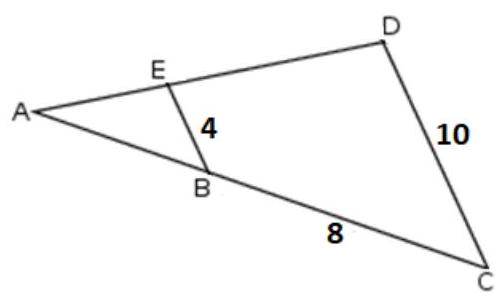
\includegraphics[max width=\textwidth, center]{2024_11_21_be8c615186155473dc68g-04}

\section*{BRUDNOPIS}
\section*{Zadanie 17. (1p)}
Dany jest trzywyrazowy ciąg geometryczny o wyrazach dodatnich: \(\left(\frac{1}{2}, \frac{x}{2}, 1\right)\). Wówczas\\
A. \(x=2\)\\
B. \(x=\sqrt{2}\)\\
C. \(x=2 \sqrt{2}\)\\
D. \(x=4\)

Zadanie 18. (1p)\\
Punkt \(S=(2,8)\) jest środkiem odcinka \(A B\), gdzie \(A=(x, 6)\) i \(B=(7,10)\) dla x równego\\
A. \(x=-3\)\\
B. \(x=3\)\\
C. \(x=-2\)\\
D. \(x=2\)

Zadanie 19. (1p)\\
Jeżeli \(x<0\), to wartość wyrażenia \(|x-4|-|x|+2 x\) jest równa\\
A. \(2 x-4\)\\
B. \(-2 x-4\)\\
C. \(-2 x+4\)\\
D. \(2 x+4\)

Zadanie 20. (1p)\\
Dany jest ciąg arytmetyczny \(\left(a_{n}\right)\), w którym różnica \(r=-3\) oraz \(a_{15}=-32\). Wówczas pierwszy wyraz tego ciągu jest równy\\
A. 8\\
B. 10\\
C. 12\\
D. 14

\section*{Zadanie 21. (1p)}
Suma wszystkich wyrazów ciągu arytmetycznego, w którym \(a_{1}=r=5\), a ostatni wyraz wynosi 250 jest równa\\
A. 6385\\
B. 6475\\
C. 6375\\
D. 6575

Zadanie 22. (1p)\\
Jeżeli wiadomo, że punkty \(A=(-1 ;-8)\) i \(B=(3 ; 4)\) należą do wykresu funkcji liniowej, to ta funkcja opisana jest wzorem\\
A. \(y=3 x-5\)\\
B. \(y=-3 x-5\)\\
C. \(y=3 x+5\)\\
D. \(y=-3 x+5\)

\section*{Zadanie 23. (1p)}
Kąt \(\alpha\) na rysunku obok ma miarę równą\\
A. \(70^{\circ}\)\\
B. \(60^{\circ}\)\\
C. \(50^{\circ}\)\\
D. \(40^{\circ}\)\\
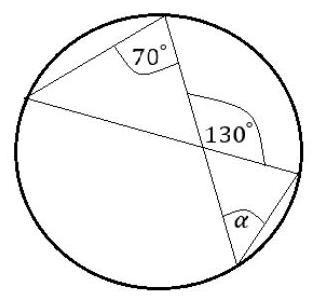
\includegraphics[max width=\textwidth, center]{2024_11_21_be8c615186155473dc68g-06}

Zadanie 24. (1p)\\
Aby otrzymać wykres funkcji \(y=5(x+1)-7\), należało wykres funkcji \(y=5 x\) przesunać\\
A. o 1 jednostkę w lewo \(i 7\) ku dołowi\\
B. o 1 jednostkę w prawo i 7 ku górze\\
C. o 1 jednostkę w prawo i 7 ku dołowi\\
D. o 1 jednostkę w lewo i 7 ku górze

Zadanie 25. (1p)\\
Funkcja kwadratowa określona jest wzorem \(f(x)=2 x^{2}+b x+1\). Jeżeli \(f(2)=5\), to\\
A. \(f(1)=-1\)\\
B. \(f(1)=1\)\\
C. \(f(1)=-2\)\\
D. \(f(1)=2\)

\section*{BRUDNOPIS}
\section*{ZADANIA OTWARTE}
Rozwiazzania zadań o numerach od 26 do 34 należy zapisać w wyznaczonych miejscach pod treścia zadania (pamiętaj o udzieleniu odpowiedzi)

Zadanie 26. (2p)\\
Rozwiąż nierówność \(x(x-1)<6\).\\

\includegraphics[max width=\textwidth, center]{2024_11_21_be8c615186155473dc68g-08}

\section*{Zadanie 27. (2p)}
Wyznacz odległość punktu \(A=(4 ;-5)\) od miejsca zerowego funkcji \(y=\frac{1}{2} x+3\).

\section*{Zadanie 28. (2p)}
Liczby 1 i -3 są miejscami zerowymi funkcji kwadratowej foraz do jej wykresu należy punkt \(P=(0,6)\). Wyznacz wzór ogólny tej funkcji.

\section*{Zadanie 29. (2p)}
Wykaż, że ciąg liczbowy o wyrazie ogólnym \(a_{n}=3 n+1\) jest ciągiem arytmetycznym.

\section*{Zadanie 30. (2p)}
Matka i córka mają łącznie 68 lat. 8 lat temu matka był trzykrotnie starsza od córki. Ile lat ma matka, a ile córka?

\section*{Zadanie 31. (2p)}
Punkt \(M\) jest środkiem boku \(A D\). Udowodnij, że pole trójkąta \(C M B\) jest połową pola trapezu \(A B C D(A B|\mid D C)\).\\
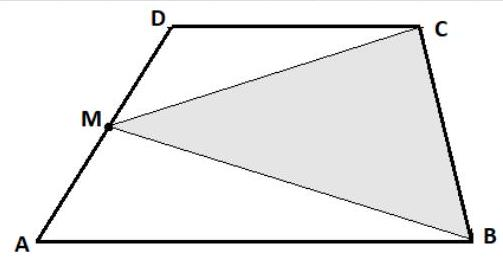
\includegraphics[max width=\textwidth, center]{2024_11_21_be8c615186155473dc68g-09}

\section*{Zadanie 32. (4p)}
Dana jest funkcja kwadratowa określona wzorem \(f(x)=-(x-2)^{2}+4\).\\
a) podaj współrzędne wierzchołka paraboli będącej wykresem tej funkcji.\\
b) podaj zbiór wartości tej funkcji.\\
c) podaj równanie osi symetrii paraboli będącej wykresem tej funkcji.\\
d) podaj wzór tej funkcji w postaci ogólnej.

\section*{Zadanie 33. (4p)}
W okręgu o promieniu 8 cm poprowadzono cięciwę AB . Długość łuku AB jest równa \(2 \pi\). Oblicz miarę kąta ostrego zawartego między cięciwą AB a styczną do okręgu w punkcie A .\\

\includegraphics[max width=\textwidth, center]{2024_11_21_be8c615186155473dc68g-10}

Zadanie 34. (5p)\\
Pierwszy wyraz ciągu arytmetycznego ( \(a_{n}\) ) jest równy 4, a suma sześciu początkowych wyrazów tego ciągu wynosi 84.\\
a) Oblicz sumę pięćdziesięciu początkowych wyrazów tego ciągu.\\
b) Dla jakiego n liczby \(a_{1}, a_{3}, a_{n}\) tworzą ciąg geometryczny?

\begin{center}
\begin{tabular}{|c|c|c|c|c|c|c|c|c|c|c|c|c|c|c|c|c|c|c|c|c|c|c|c|c|}
\hline
 &  &  &  &  &  &  &  &  &  &  &  &  &  &  &  &  &  &  &  &  &  &  &  &  \\
\hline
 &  &  &  &  &  &  &  &  &  &  &  &  &  &  &  &  &  &  &  &  &  &  &  &  \\
\hline
 &  &  &  &  &  &  &  &  &  &  &  &  &  &  &  &  &  &  &  &  &  &  &  &  \\
\hline
 &  &  &  &  &  &  &  &  &  &  &  &  &  &  &  &  &  &  &  &  &  &  &  &  \\
\hline
 &  &  &  &  &  &  &  &  &  &  &  &  &  &  &  &  &  &  &  &  &  &  &  &  \\
\hline
 &  &  &  &  &  &  &  &  &  &  &  &  &  &  &  &  &  &  &  &  &  &  &  &  \\
\hline
 &  &  &  &  &  &  &  &  &  &  &  &  &  &  &  &  &  &  &  &  &  &  &  &  \\
\hline
 &  &  &  &  &  &  &  &  &  &  &  &  &  &  &  &  &  &  &  &  &  &  &  &  \\
\hline
 &  &  &  &  &  &  &  &  &  &  &  &  &  &  &  &  &  &  &  &  &  &  &  &  \\
\hline
 &  &  &  &  &  &  &  &  &  &  &  &  &  &  &  &  &  &  &  &  &  &  &  &  \\
\hline
 &  &  &  &  &  &  &  &  &  &  &  &  &  &  &  &  &  &  &  &  &  &  &  &  \\
\hline
 &  &  &  &  &  &  &  &  &  &  &  &  &  &  &  &  &  &  &  &  &  &  &  &  \\
\hline
 &  &  &  &  &  &  &  &  &  &  &  &  &  &  &  &  &  &  &  &  &  &  &  &  \\
\hline
 &  &  &  &  &  &  &  &  &  &  &  &  &  &  &  &  &  &  &  &  &  &  &  &  \\
\hline
 &  &  &  &  &  &  &  &  &  &  &  &  &  &  &  &  &  &  &  &  &  &  &  &  \\
\hline
 &  &  &  &  &  &  &  &  &  &  &  &  &  &  &  &  &  &  &  &  &  &  &  &  \\
\hline
\end{tabular}
\end{center}

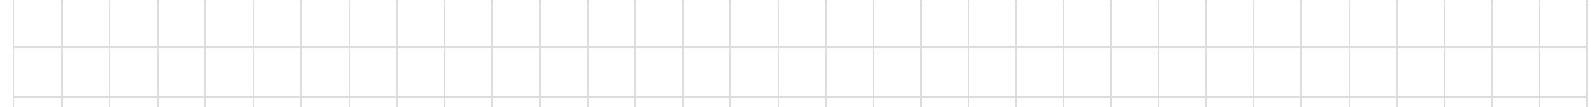
\includegraphics[max width=\textwidth, center]{2024_11_21_be8c615186155473dc68g-11(1)}\\
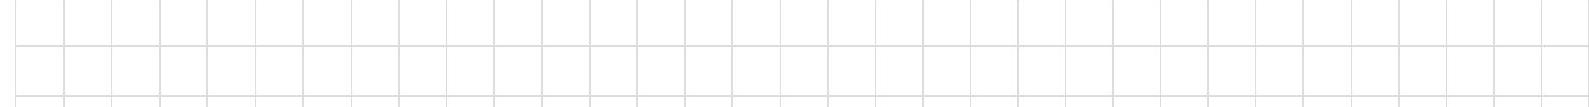
\includegraphics[max width=\textwidth, center]{2024_11_21_be8c615186155473dc68g-11(7)}\\
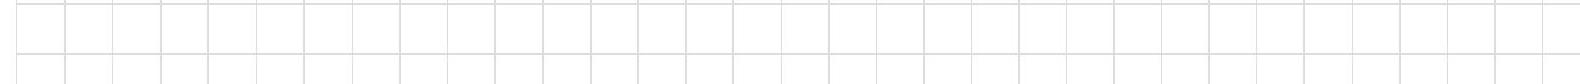
\includegraphics[max width=\textwidth, center]{2024_11_21_be8c615186155473dc68g-11(3)}


\includegraphics[max width=\textwidth]{2024_11_21_be8c615186155473dc68g-11(5)} \begin{tabular}{|l|l|l|l|l|l|l|l|l|l|l|l|l|l|l|l|l|l|}
\hline
 &  &  &  &  &  &  &  &  &  &  &  &  &  &  &  &  &  \\
\hline
 &  &  &  &  &  &  &  &  &  &  &  &  &  &  &  &  &  \\
\hline
\end{tabular}

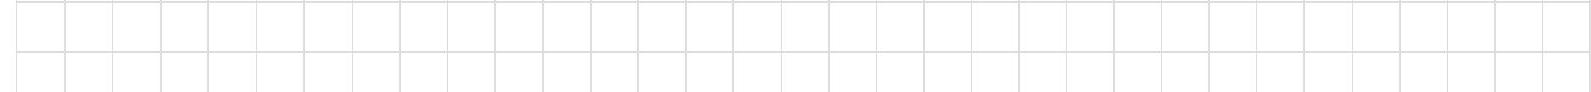
\includegraphics[max width=\textwidth, center]{2024_11_21_be8c615186155473dc68g-11(4)}\\
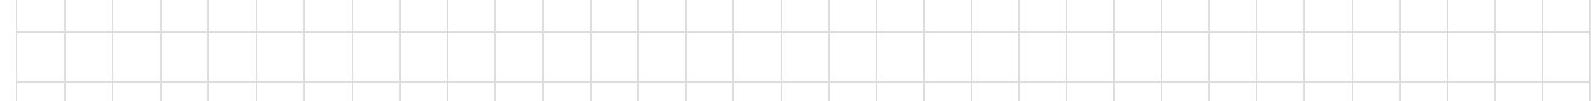
\includegraphics[max width=\textwidth, center]{2024_11_21_be8c615186155473dc68g-11(2)}

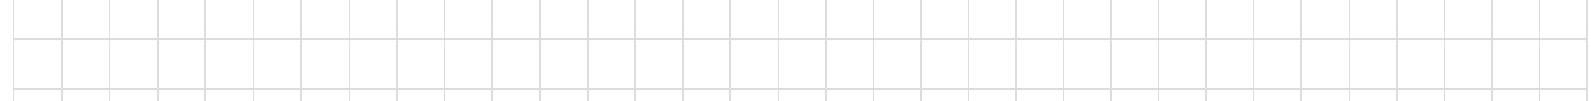
\includegraphics[max width=\textwidth]{2024_11_21_be8c615186155473dc68g-11} \textbackslash begin\{tabular\}\{ll\}\\
\textbackslash hline \\
\\
\textbackslash hline

 \begin{tabular}{|l|l|l|l|l|l|l|l|l|l|l|l|l|l|l|l|l|l|}
\end{tabular}

\textbackslash hline \& \& \& \& \& \& \& \& \& \& \& \& \& \& \& \& \& \\
\\
\textbackslash hline\\
\textbackslash end\{tabular\}

\begin{center}

\includegraphics[max width=\textwidth]{2024_11_21_be8c615186155473dc68g-11(6)}
\end{center}

\section*{BRUDNOPIS}
\section*{BRUDNOPIS}
\section*{BRUDNOPIS}
\section*{BRUDNOPIS}
KARTA ODPOWIEDZI

KOD UCZNIA \(\qquad\)\\
Wypelnia piszący

\begin{center}
\begin{tabular}{|c|c|c|c|c|}
\hline
\begin{tabular}{c}
Nr \\
zadamis \\
\end{tabular} & A & B & C & D \\
\hline
1. & \(\square\) & \(\square\) & \(\square\) & \(\square\) \\
\hline
2. & \(\square\) & \(\square\) & \(\square\) & \(\square\) \\
\hline
3. & \(\square\) & \(\square\) & \(\square\) & \(\square\) \\
\hline
4. & \(\square\) & \(\square\) & \(\square\) & \(\square\) \\
\hline
5. & \(\square\) & \(\square\) & \(\square\) & \(\square\) \\
\hline
6. & \(\square\) & \(\square\) & \(\square\) & \(\square\) \\
\hline
7. & \(\square\) & \(\square\) & \(\square\) & \(\square\) \\
\hline
8. & \(\square\) & \(\square\) & \(\square\) & \(\square\) \\
\hline
9. & \(\square\) & \(\square\) & \(\square\) & \(\square\) \\
\hline
10. & \(\square\) & \(\square\) & \(\square\) & \(\square\) \\
\hline
11. & \(\square\) & \(\square\) & \(\square\) & \(\square\) \\
\hline
12. & \(\square\) & \(\square\) & \(\square\) & \(\square\) \\
\hline
13. & \(\square\) & \(\square\) & \(\square\) & \(\square\) \\
\hline
14. & \(\square\) & \(\square\) & \(\square\) & \(\square\) \\
\hline
15. & \(\square\) & \(\square\) & \(\square\) & \(\square\) \\
\hline
16. & \(\square\) & \(\square\) & \(\square\) & \(\square\) \\
\hline
17. & \(\square\) & \(\square\) & \(\square\) & \(\square\) \\
\hline
18. & \(\square\) & \(\square\) & \(\square\) & \(\square\) \\
\hline
19. & \(\square\) & \(\square\) & \(\square\) & \(\square\) \\
\hline
20. & \(\square\) & \(\square\) & \(\square\) & \(\square\) \\
\hline
21. & \(\square\) & \(\square\) & \(\square\) & \(\square\) \\
\hline
22. & \(\square\) & \(\square\) & \(\square\) & \(\square\) \\
\hline
23. & \(\square\) & \(\square\) & \(\square\) & \(\square\) \\
\hline
24. & \(\square\) & \(\square\) & \(\square\) & \(\square\) \\
\hline
25. & \(\square\) & \(\square\) & \(\square\) & \(\square\) \\
\hline
 & Razem &  &  &  \\
\hline
\end{tabular}
\end{center}

Wypelnia sprawdzający

\begin{center}
\begin{tabular}{|c|c|c|c|c|}
\hline
\begin{tabular}{c}
Nr \\
\(\mathrm{Na}_{2}\) \\
zamia \\
\end{tabular} & X & 0 & 1 & 2 \\
\hline
26. & \(\square\) & \(\square\) & \(\square\) & \(\square\) \\
\hline
27. & \(\square\) & \(\square\) & \(\square\) & \(\square\) \\
\hline
28. & \(\square\) & \(\square\) & \(\square\) & \(\square\) \\
\hline
29. & \(\square\) & \(\square\) & \(\square\) & \(\square\) \\
\hline
30. & \(\square\) & \(\square\) & \(\square\) & \(\square\) \\
\hline
31. & \(\square\) & \(\square\) & \(\square\) & \(\square\) \\
\hline
\multicolumn{5}{|c|}{Razem} \\
\hline
\end{tabular}
\end{center}

\begin{center}
\begin{tabular}{|c|c|c|c|c|c|c|c|}
\hline
\(\underset{\text { zadania }}{\mathrm{Nr}}\) & X & 0 & 1 & 2 & 3 & 4 & 5 \\
\hline
32. & ㅁ & ㅁ & ㅁ & ■ & ㅁ & ㅁ &  \\
\hline
33. & ㅁ & ㅁ & ㅁ & ㅁ & ㅁ & ㅁ &  \\
\hline
34. & ㅁ & ㅁ & ㅁ & ■ & ㅁ & ㅁ & ㅁ \\
\hline
\end{tabular}
\end{center}

Razem\\
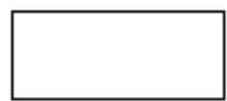
\includegraphics[max width=\textwidth, center]{2024_11_21_be8c615186155473dc68g-16}

\begin{center}
\begin{tabular}{|l|l|}
\hline
Suma punktów & Wynik w \(\%\) \\
\hline
 &  \\
 &  \\
\hline
\end{tabular}
\end{center}


\end{document}